\documentclass[TheoreticalPhy_ModB.tex]{subfiles}
\begin{document}

\newcommand{\lag}{\mathcal L}
\newcommand{\pde}[1]{\partial_{#1}}
\newcommand{\ipde}[1]{\partial^{#1}}
\newcommand{\mn}{{\mu\nu}}
\newcommand{\lr}{{L,R}}
\newcommand{\mcu}{\mathcal U}
\newcommand{\mcv}{\mathcal V}
\newcommand{\ckm}{V_{\text{CKM}}}
\newcommand{\pmns}{V_{\text{PMNS}}}
\newcommand{\upmns}{U_{\text{PMNS}}}
\newcommand{\sendC}{\overset{C}{\to}}
\newcommand{\sendP}{\overset{P}{\to}}
\newcommand{\sendT}{\overset{T}{\to}}
\newcommand{\sendCPT}{\overset{CPT}{\to}}
\newcommand{\parity}{\mathcal P}
\newcommand{\timerev}{\mathcal T}
\newcommand{\charge}{\mathcal C}



\chapter{Discrete Symmetries}

\section{The $C$, $P$ and $T$ discrete symetries for scalar, vector and Dirac fermion fields}

\textsf{Schwartz sec. 11.3-11.6; Maggiore sec. 4.2.3; Peskin sec. 3.6}\\

Up to now when discussing properties related to the Lorentz group, we have considered only local transformation near the identity, i.e. transformations in the proper orthochronus subgroup 
\[\lag_+^\uparrow\equiv\{{\Lambda^0}_0>0\,,\,\det\Lambda=1\}\]

We wanto to discuss now the role of discrete symmetries, and in particular $C$, $P$, $T$ transformations:
\begin{enumerate}[label=\textbullet]
\item $P$ and $T$ are transformations of the Lorentz group not belonging to the $\Lambda_{++}$ subgruoup
\item $C$ is a symmetry transformation that has no analogue in the non-relativistic theories, and is called \emph{charge conjugation}
\end{enumerate}

We will see that $C$, $P$, $T$ even if are symmetries of QED and QCD they are not symmetries of the SM. On the other side their combination $CPT$ is instead a symmetry of nature, as it is described by the $CPT$ theorem. 

\subsection{Discrete symmetries and scalar fields}

For simplicity we define $C$, $P$ and $T$ for a scalar fields and then we extend them for spinors and vector fields. 

\subsubsection{Parity}

Parity is a transformation that belongs to the \emph{improper orthochronus set }: ${\Lambda_0)}^0>0$, $\det\Lambda=-1$. Parity transformation is given by the inversion of space-like coordinates:
\[P=\left(\begin{array}{cccc}1 &  &  &  \\ & -1 &  &  \\ &  & -1 &  \\ &  &  & -1\end{array}\right)\qquad\text{such that}\qquad x^\mu\sendP x'^\mu=x_\mu=\left\{\begin{array}{c}x'^0=x_0 \\x'^i=x_i\end{array}\right\}=\tilde x=(x_0,-\vec x)\]

In classical mechanics parity acts as 
\[\vec x\sendP-\vec x\qquad\vec p\sendP-\vec p\qquad \vec J\sendP\vec J\]
where in the last relation we can see that axial vectors such as the angular momentum $\vec J$ are invariant under parity. We see that parity invert vectors but leaves invariant pseudovectors. 

A scalar field $\phi$ under $P$ transforms as 
\[\phi(x, t)\sendP\eta_P\phi(-x,t)=\eta_P\phi(\tilde x)\]
where $\eta_P^2=1$ and if the field $\phi$ is scalar then $\eta_P=1$, whereas if $\phi$ is a pseudoscalar then $\eta_P=-1$. The quantity $\eta_P$ is called \emph{intrinsic parity} of the scalar / pseudoscalar field. 

\begin{example}
The $\lambda(\phi^\dagger\phi)^2$ scalar field theory is $P$-invariant, indeed starting from its Lagrangian
\[\lag=\lag(x)=(\pde\mu\phi)^\dagger(\ipde\mu\phi)-m^2\phi^\dagger\phi-\frac\lambda{4!}(\phi^\dagger\phi)^2\]
(in the first equality we showed explicitly the coordinate dependence of the Lagrangian) we can see that the Lagrangian is not invariant under parity:
\[\lag(x)\sendP\lag(\tilde x)=\lag(-x,t)\neq\lag(x)\]
but the corresponding action is invariant as the measure compensates the transformation of the Lagrangian:
\[S=\int_{M_4}\de^4x\,\lag(x,t)=\int_{M_4}\de^4x\,\lag(-x,t)=S_P\]
where in the second step we performed the coordinates transformation $x\to-x$.
\end{example}

\subsubsection{Time Reversal}

Time reversal is a transformation that belong to the{ improper non-orthochronus set}: ${\Lambda_0)}^0<0$, $\det\Lambda=-1$. Parity transformation is given by the inversion of time-like coordinate:
\[T=\left(\begin{array}{cccc}-1 &  &  &  \\ & 1 &  &  \\ &  & 1 &  \\ &  &  & 1\end{array}\right)\qquad\text{such that}\qquad x^\mu\sendT x'^\mu=-x_\mu=\left\{\begin{array}{c}x'^0=-x^0 \\x'^i=x^i\end{array}\right\}=-\tilde x\]

In classical mechanics time reversal acts as 
\[\vec x\sendT\vec x\qquad\vec p\sendT-\vec p\qquad \vec J\sendT-\vec J\]
so that the helicity is left invariant, as $\vec J\cdot\vec p\sendT\vec J\cdot\vec p$.

A scalar field $\phi$ under $T$ transforms as 
\[\phi(x, t)\sendT\eta_T\phi(x,-t)=\eta_T\phi(-\tilde x)\]
where similarly to $\eta_T$ we have $\eta_T^2=1$. 

\begin{exercise}
Show that the $\lambda(\phi^\dagger\phi)^2$ theory is $T$-invariant. As in the previous example, you will see that the Lagrangian is not invariant, but the action is.
\end{exercise}

\subsubsection{Charge conjugation}

Charge conjugation is a new symmetry that cannot be described by a Lorentz transformation and has no equivalent in non-relativistic theories. 

A scalar field $\phi$ under $C$ transforms as 
\[\phi(x, t)\sendC\eta_C\phi^*(x,t)\equiv \phi^C\]
with $\eta_C^2=1$. This means that the charge conjugations transforms a (complex) field of charge $+q$ into a field of charge $-q$. 

\begin{exercise}
Show that the $\lambda(\phi^\dagger\phi)^2$ theory is $C$-invariant.
\end{exercise}
 

\subsection{Discrete symmetries and vector bosons}

$C$, $P$, $T$ transformations can be easily generalized to the vector boson case. 

A vector field $V_\mu$ under parity transform as:
\[V^\mu(x,t)\sendT\eta_PV_\mu(-x,t)=\eta_PV_\mu(\tilde x)\]
with $\eta_P^2=1$. If $\eta_P=+1$ then $V_\mu$ is a \emph{vector} while if $\eta_P=-1$ then $V_\mu$ is said a \emph{pseudovector} or \emph{axial vector}. Notice that lowering the $\mu$ index we changed the sign of the space-like components of the vector field.

A vector field $V_\mu$ under time reversal trasnforms as 
\[V^\mu(x, t)\sendT-\eta_TV_\mu( x,-t)=-\eta_TV_\mu(-\tilde x)\]
with $\eta_T^2=1$. Combining the minus sign with the lowered index we actually changed the sign of the time-like component of the vector field. 

Notice that previous transformations are more or less obvious from the Lorentz transformations of a vector:
\[x^\mu\sendP x_\mu\qquad\text{and}\qquad x^\mu\sendT-x_\mu\]
The sign difference in $V_\mu$ is due to the fact that $T$ acts as as \emph{antiunitary operator}\footnote{See Schwartz discussion in sec. 11.6.}

A vector field $V_\mu$ under $C$ transforms as 
\[V^\mu(x, t)\sendC\eta_C(V^\mu(x, t))^\dagger\]
with $\eta_C^2=1$. 
Again we define $C$ as the transformation that sends a field in its conjugated. 

\begin{exercise}
Show that YM theories (for example $SU(N)$) are invariant under $C$, $P$, and $T$. 
\end{exercise}

\subsection{Discrete symmetries and Dirac fields}

The action of discrete symmetries on spinorial fields involves also transformations of them spinorial indices, as each components of spinors have an intrinsic meaning that may be related to these transformations.  

A Dirac field under parity transforms as
\[\psi(x,t)\sendP\eta_P\gamma^0\psi(-x,t)=\eta_P\gamma^0\psi(\tilde x)=\parity\psi(\tilde x)\]
with $\eta_P^4=1$ since $\psi$ appear in terms of bilinears and $\parity=\eta_P\gamma^0$. For the adjoint field we have then
\[\bar\psi(x,t)\sendP\eta_P^*\bar\psi(-x,t)\gamma^0=\eta_P^*\bar\psi(\tilde x)\gamma^0=\bar\psi(\tilde x)\parity^\dagger\]

A Dirac field under time reversal transforms as
\[\psi(x,t)\sendT\eta_T\gamma_1\gamma_3\psi(x,-t)=\timerev\psi(-\tilde x)\]
with $\eta_T^4=1$ and $\timerev=\eta_T\gamma_1\gamma_3$ in the standard parametrization of the gamma-matrices. For the adjoint field:
\[\bar\psi(x,t)\sendT\eta_T^*\bar\psi(x,-t)\gamma_3\gamma_1=\bar\psi(-\tilde x)\timerev^\dagger\]
where $\timerev^\dagger=\timerev^{-1}$ as $\gamma_i^\dagger=-\gamma_i$ for $i=1,2,3$.

A Dirac field under charge conjugation transform as
\[\psi(x,t)\sendC\eta_Ci\gamma_2\gamma_0\bar\psi^T=\charge\bar\psi^T\equiv \psi^C\]
with $\eta_C^4=1$ and $\charge=i\eta_C\gamma_2\gamma_0$. The conjugated field transforms as
\[\bar\psi(x, t)\sendC-\psi^T\charge^\dagger=\bar\psi^C\]
Moreover one can verify the following properties:
\[\charge^\dagger=\charge^{-1}=\charge^T=-\charge\qquad\text{and}\qquad\charge^{-1}\gamma^\mu\charge=-\gamma_\mu^T\]

Notice that parity and time reversal transformations can be proven using the generators of the Lorentz group, while this is not possible for the charge conjugation. Indeed there is not an unique parametrization for the charge conjugation, and in literature different parametrization of this transformations can be found.

In the following exercize one can check that the transformations defined for $\psi$ and $\bar \psi$ under charge conjugation are consistent:

\begin{exercise}

Derive the E.M. coupled Dirac equation for $\psi^C$.\\

\textit{Solution:} Let's set $m=0$ (not need to discuss $\pm m$), then
\[i\slashed D\psi=(i\slashed \partial-q\slashed A)\psi=0\quad\longleftrightarrow\quad\bar\psi i\overset{\leftarrow}{\slashed D}=\bar\psi(i\overset{\leftarrow}{\slashed \partial}+q\slashed A)=0\]
By transposing the last equation and multiplying by $-\charge$ we obtain
\[-\charge(i\slashed\partial ^T+q\slashed A^T)\bar\psi^T=(i\slashed \partial+q\slashed A)\psi^C=0\]
Hence we see that $\psi^C$ has opposite charge of $\psi$, as $\psi^C$ obeys the Dirac equation with the sign of the charge inverted respect to the Dirac equation of $\psi$.

\end{exercise}

\section{$CPT$ transformations (and bilinears)}

As we always have to deal with bilinears of Dirac fields, let's study their properties under $C$,$P$, $T$ transformations. We define the following bilinears:
\[\begin{matrix}\text{Scalar}&\quad&S(x)=\bar\psi(x)\psi(x)\vspace{0.5cm}\\
\text{Pseudoscalar}&&P(x)=\bar\psi(x)\gamma_5\psi(x)\vspace{0.5cm}\\
\text{Vector}&&V^\mu(x)=\bar\psi(x)\gamma^\mu\psi(x)\vspace{0.5cm}\\
\text{Axial vector (or Pseudovector)}&&A^\mu(x)=\bar\psi(x)\gamma^\mu\gamma_5\psi(x)\vspace{0.5cm}\\
\text{Rank 2 antisymmetric tensor}&&T^\mn(x)=\bar\psi(x)\sigma^\mn\psi(x)&&\\\end{matrix}\]
%
Notice that the set of 16 matrices ($\gamma^\mu=4$ matrices, $\sigma^\mn=6$ matrices)
\[\Gamma=\{\id,\gamma_5,\gamma^\mu,\gamma^\mu\gamma_5,\sigma^\mn\}\]
gives a basis for all possibile $4\times4$ matrices which corresponds to all possibile Dirac bilinears.

One can verify the following transformations rules
%
\[
\begin{matrix}
  &\vline& S(x) & P(x)  & V^\mu(x)  & A^\mu(x)  & T^\mn(x)  \\
\hline\hline
P  &\vline& S(\tilde x)  & -P(\tilde x)  & V_\mu(\tilde x)  & -A_\mu(\tilde x)  & T_\mn(\tilde x)  \\
T  &\vline& S(-\tilde x)  & -P(-\tilde x)  & V_\mu(-\tilde x)  & A_\mu(-\tilde x)  & -T^\mn(-\tilde x)  \\
C  &\vline& S(x)  & P(x)  & -V^\mu(x)  & A^\mu(x)  & -T^\mn(x)  \\
CPT  &\vline& S(-x)  & P(-x)  & -V^\mu(-x)  & -A^\mu(-x)  &   T^\mn(-x) 
\end{matrix}
\]
where again $\tilde x=(x_0,-\vec x)$ and $CPT$ is the operator that combines the 3 symmetries. In the case of complex bilinears one have to add the conjugation in all the terms in the third and in the fourth rows.  
 
\begin{exercise}
Show that bilinears transform exactly as the corresponding fields.\\

\noindent
\textit{Solution:}
\[\begin{aligned}
\bar\psi(x)\psi(x)&&\sendP\quad&\bar\psi(\tilde x)\parity^\dagger\parity\psi(\tilde x)=\bar\psi(\tilde x)\psi(\tilde x)\qquad(\text{recall that }\vert\eta_P\vert^2=1\text{ and } \parity^\dagger\parity=\id)\\
\bar\psi(x)\gamma^\mu\psi(x)&&\sendP\quad&\bar\psi(\tilde x)\parity^\dagger\gamma^\mu\parity\psi(\tilde x)=\bar\psi(\tilde x)\gamma_\mu\psi(\tilde x)\qquad(\text{recall that }\gamma_0\gamma^\mu\gamma_0=\gamma_\mu)\\
\bar\psi(x)\psi(x)&&\sendC\quad&\bar\psi^C(x)\psi^C(x) = -\psi^T\charge^\dagger\charge\bar\psi^T=-\psi^T\gamma_0\psi^*=\bar\psi(x)\psi(x)\qquad(\text{recall that }\{\psi,\psi^\dagger\}=0)\\
\bar\psi(x)\gamma^\mu\psi(x)&&\sendC\quad&\bar\psi^C(x)\gamma^\mu\psi^C(x)=-\psi^T\charge^\dagger\gamma^\mu\charge\bar\psi^T=-\psi^T(-\gamma_\mu^\dagger)\bar\psi^T=-(\bar\psi\gamma_\mu\psi)^T=-\bar\psi(x)\gamma^\mu\psi(x)
\end{aligned}\]
\noindent
One can similarly prove all the other bilinears. 

\end{exercise}
 
\section{The $CPT$ theorem}

The \emph{CPT theorem} tells us that any relativistic QFT described by Hermitian and Lorentz invariant (under $\Lambda_+^\uparrow$) Lagrangian preserves the $CPT$ symmetry. 

We don't give a formal proof. But notice that the Lagrangian is a real scalar quantity, consequently
\[\lag(x)\sendCPT\lag(-x)\]
hence the Lagrangian is in general not invariant under $CPT$, whereas the CPT theorem tells us that the CPT is a symmetry of the action
\[S(x)\sendCPT S(x)\]
Moreover notice that $CPT$ theorem does not hold for $C$, $P$, $T$ independently (even though our theory may be invariant under some of these symmetries. 



\section{QED, QCD and EW properties under $C$, $P$, $T$ transformations}
\textsf{Peskin sec. 20.3}

\begin{exercise}

Show that QED and QCD are invariant under C,P,T transformations.

\noindent
\textit{Solution:}

\[\lag_{\text{QED}}=-\frac14F^{\mn}F_\mn+\bar\psi(i\slashed\partial-m)\psi-q\bar\psi\slashed A\psi\]

Under a parity transformation one has:

\[\begin{aligned}
F^\mn(x)&&\sendP\quad&F_\mn(\tilde x)&&\quad&&&A^\mu(x)&&\sendP\quad&A_\mu(\tilde x)\\
\bar\psi\gamma^\mu\psi&&\sendP\quad&\bar\psi(\tilde x)\gamma_\mu\psi(\tilde x)&&\quad&&&\partial_\mu&&\sendP\quad&\partial^\mu
\end{aligned}\]

\[\begin{aligned}
\lag_{\text{QED}}^P&=-\frac14F_\mn(\tilde x)F^\mn(\tilde x)+\bar\psi(\tilde x)(i\partial^\mu\gamma_\mu)\psi(\tilde x) - q\bar\psi(\tilde x)\gamma_\mu\psi(\tilde x)A^\mu(\tilde x)=\lag_{\text{QED}}(\tilde x)
\end{aligned}\]

\[\begin{aligned}
S_{\text{QED}}^P = \int\de^4x\,\lag_{\text{QED}}(\tilde x)=\int\de^4x\,\lag_{\text{QED}}(x)=S_{\text{QED}}
\end{aligned}\]

For the invariance under time reversal the proof is analogous.
Under a charge conjugation transformation one has:

\[\begin{aligned}
F^\mn(x)&&\sendC\quad&-F^\mn( x)&&\quad&&&A^\mu(x)&&\sendC\quad&-A^\mu( x)\\
\bar\psi\gamma^\mu\psi&&\sendC\quad&-\bar\psi( x)\gamma^\mu\psi( x)&&\quad&&&\partial_\mu&&\sendC\quad&\partial_\mu
\end{aligned}\]

\[\begin{aligned}
\lag_{\text{QED}}^C&=-\frac14F^\mn F_\mn+\bar\psi(i\slashed\partial-m)\psi-q\bar\psi\slashed A\psi
\end{aligned}\]

so $\lag_{\text{QED}}$ is invariant. 

\end{exercise}

\subsection{Violation of $CP$ of the EW sector of the Standard Model Lagrangian}

\begin{exercise}

Let's study the $\parity$ and $\charge$ transformations for chiral currents:
\[\begin{aligned}
\bar\psi_1\gamma^\mu P_L\psi_2 &&\sendP\quad&\bar\psi_1(\tilde x)\parity^\dagger\gamma^\mu P_L\parity\psi_2(\tilde x)=\bar\psi_1(\tilde x)\gamma_\mu P_R\psi_2(\tilde x)\\
\bar\psi_1\gamma^\mu P_L\psi_2&&\sendC\quad&-\psi_1^T\charge^\dagger\gamma^\mu P_L\charge\bar\psi_2^T=-\psi_1^T\charge^\dagger\gamma^\mu\charge P_L\bar\psi_2^T = \psi_1^T\gamma^{\mu,T}P_L\bar\psi_2^T=\\
&&&=-(\bar\psi_2P_L\gamma^\mu\psi_1)=-\bar\psi_2\gamma^\mu P_R\psi_1
\end{aligned}\]

Hence we have seen that under $\charge$ and $\parity$ transformations $L,R$ currents are exchanged:
\[\begin{cases}\begin{aligned}
L&&\sendP&&R\\
L&&\sendC&&-R\\
\end{aligned}\end{cases}\]

This implies that weak interactions violates both $P$ (since left-handed particles are swept with right handed ones) and $C$ (since in general right handed and left handed particles have different couplings), as we'll see better in this section.

\end{exercise}

From the first measure of Wu is known that weak interactions are $C$ and $P$ violating. Let's consider for example the charge current interactions in the mass basis
\[\lag_{\text{CC}}=\frac g{\sqrt2}\p{\bar D_L'\gamma^\mu\ckm^\dagger U_L'+\bar E_L'\gamma^\mu\pmns^\dagger N_L'}W_\mu^-+h.c.\]
By a $P$ transformation one has
\[\frac g{\sqrt2}\p{\bar D'\gamma^\mu\ckm^\dagger U'}_x\quad\sendP\quad \frac g{\sqrt2}\p{\bar D'\gamma^\mu_R\ckm^\dagger U'}_{\tilde x}\]
and similarly by $C$ transformation one has 
\[\frac g{\sqrt2}\p{\bar D'\gamma_L^\mu\ckm^\dagger U_L'}_x\quad\sendC\quad-\frac g{\sqrt2}\p{\bar U'\gamma^\mu_R\ckm^\dagger D'}_x\]
hence we see that CC Lagrangian in not invariant under $C,P$, i.e. is $\slashed C,\slashed P$. For the NC sector as $c_L\neq c_R$ one obtains the same conclusion. 
Indeed, only the QED and QCD sectors are $C$ and $P$ since they are vector like. Conversely, chiral interactions violate both $C$ and $P$.

If $\ckm\neq\ckm^\dagger$ then also $CP$ is violated in the charged current sector. Let's single out the quark current (CC)
\[\lag_{\text{CC}}=\frac g{\sqrt2}\p{\bar D'\gamma^\mu_L\ckm^\dagger U'W_\mu^-+\bar U'\gamma_L^\mu\ckm D'W_\mu^+}_x\]
where the h.c. piece has been exploited. Under a $P$ transformation the CC Lagrangian becomes 
\[\lag_{\text{CC}}^P=\frac g{\sqrt2}\p{\bar D'\gamma^\mu_R\ckm^\dagger U'W_\mu^-+\bar U'\gamma_R^\mu\ckm D'W_\mu^+}_{\tilde x}\]
Applying now a $C$ transformation one obtains
\[\lag_{\text{CC}}^{CP}=\frac g{\sqrt2}\p{\bar U'\gamma_L^\mu\ckm^\dagger D'W_\mu^++\bar D'\gamma_L^\mu\ckm U'W_\mu^-}_{\tilde x}\]
Hence $\ckm\neq\ckm^\dagger$ implies $\lag_{\text{CC}}^{CP}\neq\lag_{\text{CC}}$, i.e. the $\ckm$ and $\pmns$ phases (if non-zero) are the sources of $CP$ violation, $\slashed{CP}$. Moreover notice that all flavor and CP violation of the Standard model originates from the Yukawa sector, and this is called \emph{CKM Ansatz}. 

\begin{exercise}
Verify that the EW neutral sector beside being flavor conserving is also $CP$ conserving.
\end{exercise}

Notice that for $N=2$ families the Standard Model could not have any $\slashed{CP}$, since both $\ckm$ and $\pmns$ are real matrices (the number of phases is $(N-1)(N-2)/2$).

The $\slashed{CP}$ is a fundamental ingredient for understanding the \emph{baryon asymmetry} of the universe, i.e. why the universe is mainly made of matter rather than antimatter (CP transforms matter particles in anti-matter particles and vice versa). However the amount of $\slashed{CP}$ of the SM is not enough to explain all the universe baryon asymmetry. This problem might have two possible solutions: either the existence of new sources of $CP$ violations in theories beyond the Standard Model or new paradigm of universe, where the big bang didn't provided only energy. 

\chapter{The $\ckm$ and $\pmns$ matrices}
\textsf{Schwartz sec. 29.3.2 - 29.3.4}

The $\ckm$ and $\pmns$ matrices are $3\times3$ unitary matrices that after the spinorial phases redefinitions depend on 
\[\begin{cases}\begin{aligned}
\frac{N(N-1)}2\quad&\overset{N=3}{=}\quad3\,\text{moduli / angles}\\
\frac{(N-1)(N-2)}2\quad&\overset{N=3}{=}\quad1\,\text{phase}
\end{aligned}\end{cases}\]

\subsubsection{The standard parametrization of $\ckm$ and $\pmns$}
Let's define the following $3\times3$ rotations:
\[R_{12}(\theta_{12})=\begin{pmatrix}c_{12}&s_{12}&0\\-s_{12}&c_{12}&0\\0&0&1\end{pmatrix}\qquad
R_{13}(\theta_{13},\delta)=\begin{pmatrix}c_{13}&0&s_{13}e^{-i\delta}\\0&1&0\\-s_{13}e^{i\delta}&0&c_{13}\end{pmatrix}\qquad
R_{23}(\theta_{23})=\begin{pmatrix}1&0&0\\0&c_{23}&s_{23}\\0&-s_{23}&c_{23}\end{pmatrix}\]
where $\theta_{ij}\in[0,\pi/2)$ and $\delta\in[0,2\pi)$.Then, conventionally one defines 
\[\ckm=R_{23}(\theta_{23})\cdot R_{13}(\theta_{13},\delta)\cdot R_{12}(\theta_{12})\]
Notice that the order of rotations and the position of the $\slashed{CP}$ phase is conventional. 

For the leptonic sector there are some complications. If $\nu$s are Dirac spinors then leptonic and hadronic sectors are replicas. However, neutral $\nu$s can also be Majorana spinors and in such case two extra phases can appear in the mixing matrix:
\[\upmns=\begin{pmatrix}e^{i\alpha}&0&0\\0&e^{i\beta}&0\\0&0&1\end{pmatrix}\pmns = \phi_M(\alpha,\beta)\cdot R_{23}(\theta_{23})\cdot R_{13}(\theta_{13},\delta)\cdot R_{12}(\theta_{12})\]
where $\phi_M$ is a matrix which describes Majorana phases, and becomes the identity if we have Dirac particles. 

The $2\times4$ parameters in $\ckm$ and $\pmns$ are arbitrary parameters that have to be determined experimentally (at the same level of masses and gauge couplings). 

In the following we'll discuss the main phenomenological aspects of $\ckm$ and $\pmns$. 

\section{The quark mixing matrix $\ckm$}

The $\ckm$ entries are usually dubbed with the nouns of the up-down quarks it connects:
\[\ckm\equiv R_LS_L^\dagger=\begin{pmatrix}V_{ud}&V_{us}&V_{ub}\\V_{cd}&V_{cs}&V_{cb}\\V_{td}&V_{ts}&V_{tb}\end{pmatrix}=R_{23}\cdot R_{13}\cdot R_{12}\]

To determine the $\ckm$ entries one has to measure the corresponding meson/baryon decays. For instance, the measure of $V_{ud}$ can be done through the measurement of the $\beta$-decay amplitude:
\onlyinmainfile{
\[\begin{tikzpicture}[baseline=(u3)]
	\begin{feynman}[large]
		\vertex(u1){$u$};
		\vertex[below=2em of u1](d1){$d$};
		\vertex[below=2em of d1](d2){$d$};
		\vertex[right=2cm of u1](a1);
		\vertex[right=2cm of d1](a2);
		\vertex[right=2cm of d2](a3);
		\vertex[right=2cm of a1](a);
		\vertex[above=0.7cm of a](u2){$u$};
		\vertex[below=2em of u2](d3){$d$};
		\vertex[below=2em of d3](u3){$u$};
		\vertex[below=2cm of a](w);
		\vertex[above right=1cm of w](e){$e^-$};
		\vertex[below right=1cm of w](n){$\bar\nu_e$};
		\diagram*{
			(u1)--[fermion](a1)--[fermion](u2),
			(d1)--[fermion](a2)--[fermion](d3),
			(d2)--[fermion](a3)--[fermion](u3),
			(a3)--[gluon,edge label'={$W^-$}](w),
			(n)--[fermion](w)--[fermion](e),
		};
		\draw [decoration={brace}, decorate] (d2.south west) -- (u1.north west) node [pos=0.5, left] {\(n\)};
		\draw [decoration={brace}, decorate] (u2.north east) -- (u3.south east) node [pos=0.5, right] {\(p\)};
	\end{feynman}
\end{tikzpicture}
\qquad\propto\vert V_{ud}\vert ^2g^4\]
while the measurement of $V_{us}$ can be done observing the $K^0$ decay:
\[\begin{tikzpicture}[baseline=(s)]
	\begin{feynman}[large]
		\vertex(d1){$\bar d$};
		\vertex[below=2em of d1](s){$s$};
		\vertex[right=2cm of d1](a1);
		\vertex[right=2cm of s](a2);
		\vertex[right=2cm of a2](a);
		\vertex[above=1cm of a](d2){$\bar d$};
		\vertex[below=2em of d2](u){$u$};
		\vertex[below=1.1cm of a](w);
		\vertex[above right=1cm of w](e){$e^-$};
		\vertex[below right=1cm of w](n){$\bar\nu_e$};
		\diagram*{
			(d1)--[fermion](a1)--[fermion](d2),
			(s)--[fermion](a2)--[fermion](u),
			(a2)--[gluon,edge label'={$W^-$}](w),
			(n)--[fermion](w)--[fermion](e),
		};
		\draw [decoration={brace}, decorate] (s.south west) -- (d1.north west) node [pos=0.5, left] {\(n\)};
		\draw [decoration={brace}, decorate] (d2.north east) -- (u.south east) node [pos=0.5, right] {\(p\)};
	\end{feynman}
\end{tikzpicture}
\qquad\propto\vert V_{us}\vert ^2g^4\]
}

Notice that inside mesons / baryons the quarks are in the mass eigenstates, so we have to use the mass basis Feynman rules. 
From all available experimental determinations we obtain the following matrix, where phases are omitted:

\[\vert\ckm\vert = \begin{pmatrix}0.97446\pm0.00010&0.22452\pm0.00044&0.00365\pm0.00012\\0.22438\pm0.00044&0.97359\pm0.00010&0.04214\pm0.00076\\0.00856\pm0.00024&0.04133\pm0.00074&0.999105\pm0.000032\end{pmatrix}\]
Notice that the matrix is quasi diagonal (hence the angles of rotation are small) and is quasi-symmetric. In particular it gives the following determination of the standard parameters
\[\begin{aligned}\theta_{12}&=13.02^\circ\pm0.04^\circ&&&\theta_{23}&=2.36^\circ\pm0.08^\circ\\
\theta_{13}&=0.20^\circ\pm0.02^\circ&&&\delta_{(13)}&=69^\circ\pm5^\circ\end{aligned}\]
Since $\delta\neq0,\pi$ we see that $\ckm$ violates the $CP$ symmetry. 

\subsection{The Wolfestein parametrization}

From the experimental results one can notice a well defined pattern/hierarchy between the coefficients $V_{ij}$ in $\ckm$:
\begin{enumerate}
	\item the diagonal elements are $O(1)$
	\item elements $V_{12}$ and $V_{21}$ are $O(10^{-1})$,
	\item elements $V_{23}$ and $V_{32}$ are $O(10^{-2})$,
	\item elements $V_{13}$ and $V_{31}$ are $O(10^{-3})$,
\end{enumerate}
and, since 
\[R_{23}(\theta_{23})\cdot R_{13}(\theta_{13},\delta)\cdot R_{12}(\theta_{12})=
\begin{pmatrix}c_{12}c_{13}&s_{12}s_{13}&s_{13}e^{-i\delta}\\
\bullet&\bullet&s_{23}c_{13}\\
\bullet&\bullet&c_{23}c_{13}\end{pmatrix}\]
(where $\bullet$ denots more complex terms, omitted), consequently
\[s_{13} \ll s_{23} \ll s_{12} < 1\]

To made explicit this hierarchical structure on $\ckm$ it is often convenient  to use the 
\textbf{Wolfenstein parametrization}:
\[s_{12}=\frac{\vert V_{us}\vert}{\p{\vert V_{ud}\vert^2+\vert V_{us}\vert^2}^{1/2}}\equiv\lambda
\qquad
s_{23}=\lambda\frac{\vert V_{cb}\vert}{\vert V_{us}\vert}\equiv A\lambda^2
\qquad
s_{13}e^{i\delta}= V_{ub}^*\equiv A\lambda^3(\rho+i\eta)\]
Then $\ckm$ can be written in terms of the 4 independent parameters $(A,\lambda,\rho\eta)$ as
\[\ckm=\begin{pmatrix}1-\frac{\lambda^2}2&\lambda&A\lambda^3(\rho-i\eta)\\
-\lambda&1-\frac{\lambda^2}2&A\lambda^2\\
A\lambda^3(1-\rho-i\eta)&A\lambda^2&1\end{pmatrix}+O(\lambda^4)\]

\begin{exercise} 
Prove that up to $O(\lambda^4)$ the $\ckm$ matrix is approximated by the Wolfenstein parametrization.
\end{exercise}

If we write $\lambda=s_{12}\equiv\sin(\theta_C)$ then the angle $\theta_C$ is said \textbf{Cabibbo angle}. Usually we call $\lambda$ itself the Cabibbo angle.

Experimental fits give the following determination of the Wolfenstein parameters
\[\begin{aligned}
\lambda&=0.22453\pm0.00044 &&\quad&&A&=0.836\pm0.015\\
\rho&=0.122\pm0.018&&\quad&&\eta&=0.355\pm0.012\end{aligned}\]

The hierarchy of $\ckm$ is then explicitated in terms of the small Cabibbo angle:
\begin{enumerate}
	\item the diagonal elements are $O(1)$
	\item elements $V_{12}$ and $V_{21}$ are $O(\lambda)$,
	\item elements $V_{23}$ and $V_{32}$ are $O(\lambda^2)$,
	\item elements $V_{13}$ and $V_{31}$ are $O(\lambda^3)$.
\end{enumerate}

\subsection{$\ckm$ and unitary triangles}

One of the best constraints of $\ckm$ comes from imposing unitary conditions. Notice that \emph{CKM ansatz} says that all flavor and CP violation in the SM comes from $\ckm$ (and $\pmns$). By construction $\ckm$ (and $\pmns$) is a  unitary $3\times3$ matrix:
\[\ckm^\dagger\ckm=\id_{3\times3}=\ckm\ckm^\dagger\]
Multiplying rows and columns of a $3\times3$ unitary matrix one obtains 12 relations:
\begin{enumerate}
	\item 6 normalization conditions:
	\[\sum_{i=1}^3\vert V_{ij}\vert^2=1=\sum_{j=1}^3\vert V_{ij}\vert^2\]
	\item 6 orthogonality conditions
	\[\sum_{i=1}^3V_{ij}V_{ik}^*=0=\sum_{j=1}^3V_{ij}V_{kj}^*\]
\end{enumerate}

Orthogonality conditions are particularly useful as one can precisely check the Standard Model Yukawa sector and eventually have hints of physics beyond the SM. 

Orthogonality relations have a useful graphical representation. Lets consider $\sum_{i=1}^3V_{ij}V_{ik}^*=0$ with $j=1,k=3$. This relation corresponds to multiply the $3^{\text{rd}}$ row of $\ckm^\dagger$ with the $1^{\text{st}}$ columns of $\ckm$:
\[V_{ud}V_{ub}^*+V_{cd}V_{cb}^*+V_{td}V_{tb}^*=0=R_u+R_c+R_t\]
In the complex space the values $R_u,R_c,R_t$ can be regarded as vectors whose sum vanishes, so pictorially the unitary conditions can be represented by a triangle whose edges are these three vectors:          

\[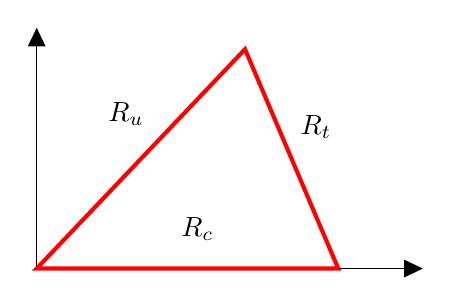
\begin{tikzpicture}[x=0.75pt,y=0.75pt,yscale=-1,xscale=1]
\draw    (110.5,210) -- (110.5,97) ;
\draw [shift={(110.5,94)}, rotate = 450] [fill=black][line width=0.08][draw opacity=0] (8.93,-4.29) -- (0,0) -- (8.93,4.29) -- cycle ;
\draw    (110.5,210) -- (293.5,210) ;
\draw [shift={(296.5,210)}, rotate = 180] [fill=black][line width=0.08][draw opacity=0] (8.93,-4.29) -- (0,0) -- (8.93,4.29) -- cycle    ;
\draw  [color=red,draw opacity=1 ][line width=1.5]  (255.78,210) -- (110.5,210) -- (210.88,104.34) -- cycle ;
\draw (143.72,128.69) node [anchor=north west][inner sep=0.75pt][align=left] {$R_{u}$};
\draw (236.44,134.95) node [anchor=north west][inner sep=0.75pt][align=left] {$R_{t}$};
\draw (178.89,184.02) node [anchor=north west][inner sep=0.75pt][align=left] {$R_{c}$};
\end{tikzpicture}\]

\noindent
In the Wolfenstein parametrization one has
\[\begin{cases}
R_u=V_{ud}V_{ub}^*=\p{1-\frac{\lambda^2}2}\p{A\lambda^3}\p{\rho+i\eta}\simeq A\lambda^3(\rho+i\eta)\\
R_c=V_{cd}V_{cb}^*=-A\lambda^3\\
R_t=V_{td}V_{tb}=A\lambda^3(1-\rho-i\eta)
\end{cases}\]
hence by renormalizing with respect to $\vert R_c\vert$ the previous triangle reads     

\[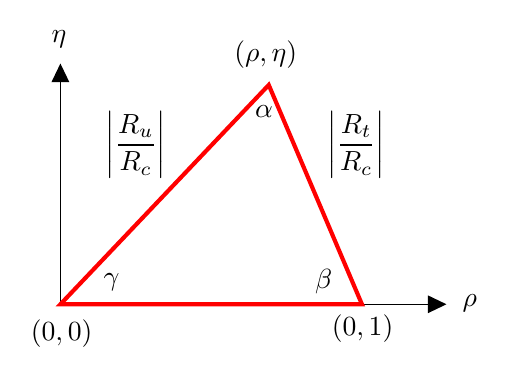
\begin{tikzpicture}[x=0.75pt,y=0.75pt,yscale=-1,xscale=1]
\draw    (110.5,210) -- (110.5,97) ;
\draw [shift={(110.5,94)}, rotate = 450] [fill=black][line width=0.08][draw opacity=0] (8.93,-4.29) -- (0,0) -- (8.93,4.29) -- cycle    ;
\draw    (110.5,210) -- (293.5,210) ;
\draw [shift={(296.5,210)}, rotate = 180] [fill=black][line width=0.08][draw opacity=0] (8.93,-4.29) -- (0,0) -- (8.93,4.29) -- cycle    ;
\draw  [color=red,draw opacity=1 ][line width=1.5]  (255.78,210) -- (110.5,210) -- (210.88,104.34) -- cycle ;
\draw (131,116) node [anchor=north west][inner sep=0.75pt]   [align=left] {$\displaystyle\left|\frac{R_{u}}{R_{c}} \right|$};
\draw (240,214) node [anchor=north west][inner sep=0.75pt]   [align=left] {$(0,1)$};
\draw (95,216) node [anchor=north west][inner sep=0.75pt]   [align=left] {$(0,0)$};
\draw (193,82) node [anchor=north west][inner sep=0.75pt]   [align=left] {$(\rho ,\eta )$};
\draw (238,116) node [anchor=north west][inner sep=0.75pt]   [align=left] {$\displaystyle \left|\frac{R_{t}}{R_{c}} \right|$};
\draw (303,204) node [anchor=north west][inner sep=0.75pt]   [align=left] {$ \rho $};
\draw (105,77) node [anchor=north west][inner sep=0.75pt]   [align=left] {$ \eta $};
\draw (203,113) node [anchor=north west][inner sep=0.75pt]   [align=left] {$ \alpha $};
\draw (232,192) node [anchor=north west][inner sep=0.75pt]   [align=left] {$ \beta $};
\draw (130,194) node [anchor=north west][inner sep=0.75pt]   [align=left] {$ \gamma $};
\end{tikzpicture}\]

The measure of the 2 sides (the third is chosen to be 1 by normalization) and the 3 angles provides a stringent check of the unitary of $\ckm$ 
\[\begin{aligned}
\left\vert\frac{R_u}{R_c}\right\vert&=\left\vert\frac{V_{ud}V_{ub}^*}{V_{cd}V_{cb}^*}\right\vert\simeq\frac1\lambda\left\vert\frac{V_{ub}}{V_{cb}}\right\vert=[\rho^2+\eta^2]^{1/2}\\
\left\vert\frac{R_t}{R_c}\right\vert&=\left\vert\frac{V_{td}V_{tb}^*}{V_{cd}V_{cb}^*}\right\vert\simeq\frac1\lambda\left\vert\frac{V_{td}}{V_{cb}}\right\vert=[(1-\rho)^2+\eta^2]^{1/2}\\
\alpha&=\operatorname{Arg}\left[-\frac{V_{td}V_{tb}^*}{V_{ud}V_{ub}^*}\right]\\
\beta&=\operatorname{Arg}\left[-\frac{V_{cd}V_{cb}^*}{V_{td}V_{tb}^*}\right]\\
\gamma&=\operatorname{Arg}\left[-\frac{V_{ud}V_{ub}^*}{V_{cd}V_{cb}^*}\right]\\
\end{aligned}\]
together with the constraints $\alpha+\beta+\gamma=\pi$. In terms of $\rho$ and $\eta$ one can also write
\[\sin2\beta=\frac{2\eta(1-\rho)}{(1-\rho)^2+\eta^2}
\qquad
\sin2\gamma=\frac{2\eta\rho}{\rho^2+\eta^2}\]
which shows that if $\eta=0$ then $\beta=\gamma=0$. If either $\sin2\beta\neq0$ or $\sin2\gamma\neq0$ then $\eta\neq0$ and we have a CP violation. 

By measuring all the $\ckm$ elements (and all their combinations) we over-constrained the unitary triangle and one have a consistency check. Any deviation from the unitary constraints is would be a  signal of new physics coming out. 

\section{The lepton mixing matrix $\pmns$}

If neutrinos are Dirac fermions, all the discussion done for the quarks on the mixing matrix can be extended to the $\pmns$:
\[\pmns\equiv R_{23}(\theta_{23})R_{13}(\theta_{13},\delta)R_{12}(\theta_{12})\]
However the fact that neutrinos are practically massless makes very complicated the measure of the $\pmns$ entries. Let's recall the $\lag_{\text{CC}}$ interaction term in the mass basis:
\[\bar N_L'\gamma^\mu\pmns E_L'W_\mu^++h.c. = \sum_{i,j}\bar\nu_i'V_{ij}e_j'W_\mu^++h.c.\]
and let's make the following definitions:
\begin{enumerate}
	\item $\nu_i'\equiv(\nu_1,\nu_2,\nu_3)$ are \textbf{neutrino mass eigenstates};
	\item $\nu_\alpha\equiv(\nu_e,\nu_\mu,\nu_\tau)$ are \textbf{neutrino flavor eigenstates};
	\item $\ell_i'\equiv(e,\mu,\tau)$ are the physical leptons we defined in QED (mass eigenstates)
\end{enumerate}
 
Let's consider the $W_\mu^+\longrightarrow e^+\nu_i$, the $W^+$ decay into physical (mass) states. If we are not able to identify $\nu$s mass eigenstates the process we measure is 

\[\begin{tikzpicture}[baseline=(a)]
	\begin{feynman}[medium]
		\vertex(a);
		\vertex[left=of a](w){$W^+$};
		\vertex[above right=of a](n){$\nu_i$, {\footnotesize $i=1,2,3$}};
		\vertex[below right=of a](e){$e^+$};
		\diagram*{
			(w)--[gluon](a),
			(e)--[fermion](a)--[fermion](n),
		};
	\end{feynman}
\end{tikzpicture}
= \p{\sum_{i=1}^3\bar\nu_iV_{ie}}\gamma_L^\mu \,e^+W_\mu^+
\]
since we are not able to identify which neutrino is produced in the final state. In other words we measure only the interaction between the electron and the $\nu_e$ flavor eigenstate, which means:
\[\nu_e\equiv\sum_{i=1}^3V_{ei}^*\nu_i\]
while more in general
\[\nu_\alpha\equiv\sum_{i=1}^3V_{\alpha i}^*\nu_i
\qquad
\text{where } \alpha=(e,\mu,\tau)\]

This means that neutrinos are produced and detected only as flavor eigenstates.. 

\[\begin{tikzpicture}[baseline=(a)]
	\begin{feynman}
		\vertex(a);
		\vertex[left=of a](w){$W^+$};
		\vertex[above right=of a](n){$\nu_e$};
		\vertex[below right=of a](e){$e^+$};
		\diagram*{
			(w)--[gluon](a),
			(e)--[fermion](a)--[fermion](n),
		};
	\end{feynman}
\end{tikzpicture}
=\bar\nu_e\gamma_L^\mu e^+W_\mu^+\]

Remember that if $m_{\nu_i}=0$ then $\pmns=\id$. We just seen that $\pmns$ parameters cannot be measured in weak interactions (such as $W^\pm$ decays etc.).

\subsection{Neutrino oscillations (in vacuum)}

The only way we can at present have access to neutrinos (differences of masses and) mixing is thanks to \textbf{neutrino oscillations}. To describe this phenomena, one can use pure quatum mechanics description of waves propagations. Let's suppose that flavors are different than mass eigenstates:
\begin{enumerate}
	\item $\ket{\nu_\alpha} \equiv (\nu_e,\nu_\mu,\dots)$ is the \textbf{flavor basis},
	\item $\ket{\nu_i}\equiv(\nu_1,\nu_2,\dots)$ is the \textbf{mass basis}.
\end{enumerate}
The flavor state can be described as a linear combination of mass eigenstates
\[\ket{\nu_\alpha}=\sum U_{\alpha i}\ket{\nu_i}\]
Notice that if neutrinos are Majorana particles then $U=\phi_M^\dagger\cdot\pmns^\dagger$. However as we will see neutrino oscillations do not depend on the Majorana phases $\phi_M$. 

Suppose that a $\nu_\alpha$ is produced at $t=0$. We want to measure how many $\nu_\beta$ are detected at a $t=t_0\neq0$. The evolution of $\nu_\alpha$ can be obtained by solving the $\nu_i$ Schrödinger equation
\[\begin{cases}
	i\frac\de{\de t}\ket{\nu_i}=\mathcal H\ket{\nu_i}=E_i\ket{\nu_i}\\
	\ket{\nu_i(t)}=\exp{-iE_it}\ket{\nu_i(0)}
\end{cases}\]
together with 
\[\ket{\nu_\alpha(t)}=\sum U_{\alpha i}\exp{-iE_it}\ket{\nu_i(0)}\]
 
The probability to detect a flavor $\beta$ (by weak interactions) at a certain $t\neq0$ is then
\[\begin{aligned}
P_{\alpha\beta}(t)&\equiv\left\vert\braket{\nu_\beta}{\nu_\alpha(t)}\right\vert^2
=\Big\vert\sum_iU_{\alpha i}\exp{-iE_it}\braket{\nu_\beta}{\nu_i(0)}\Big\vert^2\\
&=\Big\vert\sum_{ij}U_{\beta j}^*\exp{-iE_it}U_{\alpha i}\braket{\nu_j(0)}{\nu_i(0)}\Big\vert^2
=\Big\vert\sum_iU_{\beta i}^*\exp{-iE_it}U_{\alpha i}\Big\vert^2
\end{aligned}\]

\begin{exercise}
Show that $P_{\alpha\beta}$ does not depend on the diagonal Majorana phases matrices $\phi_M$.
\end{exercise}

The general probability formula can be easily obtained as follows
\[\begin{aligned}
P_{\alpha\beta}&=\Big\vert\sum_i U_{\beta i}^*\exp{-iE_it}U_{\alpha i}\Big\vert^2
=\sum_{ij}\exp{-i(E_i-E_j)t}U_{\beta i}^*U_{\alpha_i}U_{\beta j}U_{\alpha j}^*\\
&=\sum_{ij}W_{\alpha\beta}^{ij}\exp{-i(E_i-E_j)t}
=\sum_{i=j}W_{\alpha\beta}^{ij}+\sum_{i<j}\p{\Re\p{W_{\alpha\beta}^{ij}}\cos(\Delta E_{ij}t)+\Im\p{W_{\alpha\beta}^{ij}}\sin(\Delta E_{ij})}\\
&=\sum_{i=j}W_{\alpha\beta}^{ij}+\sum_{i\neq j}\Re\p{W_{\alpha\beta}^{ij}}-4\sum_{i<j}\Re\p{W_{\alpha\beta}^{ij}}\sin^2\p{\frac{\Delta E_{ij}t}2}+2\sum_{i<j}\Im\p{W_{\alpha\beta}^{ij}}\sin(\Delta E_{ij}t)
\end{aligned}\]
where $W_{\alpha\beta}^{ij}=U_{\beta i}^*U_{\alpha_i}U_{\beta j}U_{\alpha j}^*$. The fist two terms in the last line give $\delta_{\alpha\beta}$ due to unitarity of $U_{\alpha i}$. The other pieces can be rewritten using the following relation:
\[\Delta E_{ij}=E_i-E_j\simeq\p{p+\frac12\frac{m_1^2}p}-\p{p+\frac12\frac{m_2^2}p}\simeq\frac{\Delta m_{ij}^2}{2E}\]
where $p\simeq E$ as $m_i\ll p$ (notice that the 3 mass eigenstates have same value  fo $p$, since we are propagating just one wave). As $c=1$ we can also replace $t \rightarrow L$. The probability of oscillations then reads
\[P_{\alpha\beta}=\delta_{\alpha\beta}-4\sum_{i<j}\Re\p{W_{\alpha\beta}^{ij}}\sin^2\p{\frac{\Delta m_{ij}^2L}{4E}}\pm2\sum_{i<j}\Im\p{W_{\alpha\beta}^{ij}}\sin\p{\frac{\Delta m_{ij}^2L}{2E}}\]
The $\pm$ sign refers either to neutrino ($+$) or antineutrino ($-$). In fact under CP one has $U\rightarrow U^\dagger$ and so $W_{\alpha\beta}^{ij}\rightarrow W_{\alpha\beta}^{ij\,*}$, then the minus sign comes out due to $\Im(\bullet)$ after the conjugation.

Measuring the oscillation probability one has access to 
\begin{enumerate}
	\item $\pmns$ parameters through $W_{\alpha\beta}^{ij}$,
	\item $\Delta m_{ij}^2$ mass difference.
\end{enumerate}
The explicit 3 neutrinos oscillation probability without any approximation is quite large. We can also show this result for 2 families. 

\begin{exercise}

Derive $P_{\alpha\beta}$ for two neutrinos.

\noindent
\textit{Solution:}

The $\pmns$ matrix for $N=2$ depends only on 1 angle and 0 phases:
\[\begin{pmatrix}\nu_e\\\nu_\mu\end{pmatrix}=\begin{pmatrix}U_{e1}=c_\theta&U_{e2}=s_\theta\\U_{\mu1}=-s_\theta&U_{\mu2}=c_\theta\end{pmatrix}\begin{pmatrix}\nu_1\\\nu_2\end{pmatrix}
\quad\rightarrow\quad
\begin{cases}\nu_e(+)=c_\theta e^{-iE_1t}\nu_1+s_\theta e^{-iE_2t}\nu_2\\
\nu_\mu(+)=-s_\theta e^{-iE_1t}\nu_1+c_\theta e^{-iE_2t}\nu_2\end{cases}\]

The $P(\nu_\mu\rightarrow\nu_e)$ appearance probability is 
\[\begin{aligned}
P_{21} &= \vert\braket{\nu_e}{\nu_\mu(+)}\vert^2
=\left\vert -s_\theta c_\theta e^{-iE_1t}+s_\theta c_\theta e^{-iE_2t}\right\vert^2
=2s_\theta^2 c_\theta^2-2s_\theta^2c_\theta^2\cos(\Delta E_{12}t)\\
&= 2s_\theta^2 c_\theta^2-2s_\theta^2 c_\theta^2+4s_\theta^2 c_\theta^2\sin^2\p{\frac{\Delta E_{12}t}2}
=\sin^22\theta\sin^2\p{\frac{\Delta m_{12}^2L}{4E}}
\end{aligned}\]

The $P(\nu_\mu\rightarrow\nu_e)$ disappearance probability is, due to unitarity (conservation of probability),
\[P_{11}=\vert\braket{\nu_e}{\nu_e(+)}\vert^2=1-P_{21}=1-\sin^22\theta\sin^2\p{\frac{\Delta m_{12}^2L}{4E}}\]

As for $N=2$ the matrix $\pmns$ is real, it is immediate to recover the antineutrino probability
\[\begin{cases}\begin{aligned}
P(\bar\nu_\mu\rightarrow\bar\nu_e)=P(\nu_\mu\rightarrow\nu_e)\\
P(\bar\nu_e\rightarrow\bar\nu_e)=P(\nu_e\rightarrow\nu_e)
\end{aligned}\end{cases}\]

\end{exercise}

\subsection{Experimental determination of $\pmns$}

One can use many sources of neutrino fluxes:
\begin{enumerate}
	\item solar neutrinos (from the Sun are mainly $\nu_e$),
	\item atmospherical neutrinos (from cosmic rays are mainly $\nu_\mu$),
	\item accelerators and reactors (all the three types $\nu_e,\nu_\mu,\nu_\tau$).
\end{enumerate}

By measuring all appearance and disappearance probabilities of neutrino oscillations one can obtain the following results:
\begin{enumerate}
	\item $\Delta m_{21}^2 = \Delta m_{\text{Sun}}^2=(7.53\pm0.18)\times 10^{-5}$eV 
	\item $\Delta m_{31}^2=\Delta m_{\text{Atm}}^2=(2.44\pm0.06)\times 10^{-3}$eV
	\item $\sin^2(2\theta_{12})=0.846\pm0.021$
	\item $\sin^2(2\theta_{23})>0.92$
	\item $\sin^2(2\theta_{13})=0.093\pm0.008$
	\item $\delta$ is not determined yet
\end{enumerate}
Notice that angles $\theta_{12}$ and $\theta_{23}$ are big, while $\theta_{13}$ is small. Since the values for $\pmns$ are different from values of $\ckm$, in this case we cannot use Wolfenstein parametrization. 

If $m_{\nu_i}=0$ then one could not have observed neutrino oscillations (neither if $m_{\nu_i}=m_{\nu_j}$). If the mass basis is the same as the flavor basis we should have $\theta_{ij}=0$ as $\pmns=\id$ and all $P(\nu_\alpha\rightarrow\nu_\beta)=0$ for $\alpha\neq\beta$. This prove that neutrinos are massive, and their masses are different. 
	


\end{document}